\chapter{Introduction}

Autonomous surface vehicles (ASV) has a range of applications such as environmental monitoring \cite[p. 745]{MAHsieh}, meteorological data collection, marine biological research and surveillance \cite[p. 8-10]{FFahimi}.
Designing an ASV raises a some interesting control challenges, varying between the intended functionalities.

One use case for a small ASV is shown in \autoref{fig:USVforRescue}. This is a solution for search and rescue missions in floods. It can be dangerous and difficult for rescuers to search in flooded areas. A drone is able to reach otherwise inaccessible places and provides better vision horizons than an ASV would. The drone however has short battery life, which limits the reach and duration of the mission.
%
\begin{figure}[H]
  \vspace{3mm}
  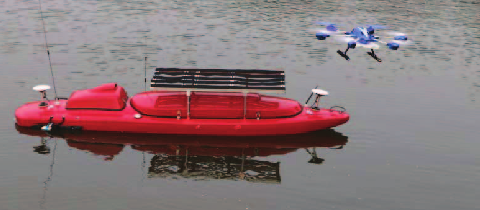
\includegraphics[width=0.62\textwidth]{figures/USVforRescue.pdf}
  \caption{An air-surface system for search in flooded areas under search and rescue missions.\cite{JZhang}}
  \label{fig:USVforRescue}
\end{figure}
\vspace{-6mm}
%
Here the ASV provides long battery life and by carrying the drone, until needed for improved overview, extends reach and duration of each mission.\cite{JZhang}


%%%%%%%%%%Survey%%%%%%%%%%

Another application is for automated survey of an area.
Bathymetric measurements can be used for efficient and safe guidance of marine vessels in shallow waters. 
It is also interesting when studying biological oceanography where it i.e. can help in deciding which areas to protect for preservation of sea life \cite{NOService}. 

For some types of survey it is required for the ASV to maintain it's GPS position while preforming measurements. 
This requires the system to be able to estimate and counteract external forces, applied to the vessel, keeping it still. 

%A basic functionality of a ASV is to follow a route. 
%This enables to ASV to arrive at a survey side and to preform measurements along a path. 
%%%% https://pdfs.semanticscholar.org/ce94/01a72e78b314f5d2fbbce66f56b217acef1c.pdf
In volcanic countries observations are carried out by volcanologists to provide forecasts and warnings. One observation target is crater lakes. Flash floods and hydrovolcanic explosions can be caused by such lakes. Observing these can help providing information when precautions must be taken and potential evacuation planned.\cite{AWatanabe}
%
\begin{figure}[H]
  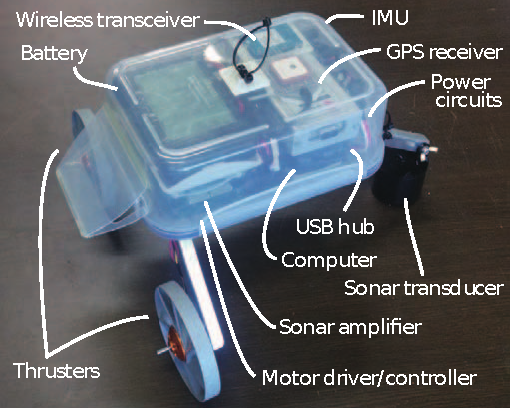
\includegraphics[width=0.35\textwidth]{figures/volcanicLakeUSVwLabels.pdf}
  \caption{Small ASV for taking bathymetric measurements in the Mt. Zao Okama Crater Lake in Japan.\cite{AWatanabe}}
  \label{fig:volcanicLakeUSVwLabels}
\end{figure}
\vspace{-6mm}
%
The small ASV seen in \autoref{fig:volcanicLakeUSVwLabels} is designed to take bathymetric measurements of such lakes and eliminate the need to endanger humans in the process.\cite{AWatanabe}

The USV is made specifically for the Mt. Zao Okama Crater Lake in Japan, where it replaces the need for a manned canoe to enter the volcanic lake situated in high
altitude, strong wind, and restricted area. The bathymetric measurements are used to indicate the amount of water, crater wall caving, and volcanic upthrusts in the lake.\cite{AWatanabe}

An example of a system designed to preform such task is [Insert solar vessel here]. 
%This implementation achieves such functionality is through a two layer design. 
%An inner controller manipulates the dynamics of the system, while an outer controller is responsible for steering the route through the inner controller. 
It is able to detect and avoid obstacles in the water, while preforming high precision bathymetric measurements. 
The vessel uses solar cells, which gives the added challenge of controlling the vessel at low speeds, to prevent battery usage during operation for longevity. 
This allows the vessel to autonomously survey relatively large areas without needing to recharge.
 


%
%one strength of an ASV is that it can map out an entire stream, whereas manual measurements typicaly will be cumbersome and low in mapping resolution due to accessibility of the stream and time constraints/cost.\\
%for marine survey it can be useful as it can enter narrower and more shallow waters than larger manned vessels would be able to.\\
%the military has also been using ASV's for surveillance.
In this project, the design and implementation of a ASV able to preform bathymetric measurement will be described. 
This will be done using the aauship platform supplied for this project by Aalborg university. 
%In this project the focus is first and foremost the control design, which will be realized with focus on bathymetric measurements. This will constitute a basis for setting up requirements for precision which will determine important parameters in the control design.
